\documentclass[12pt,a4paper]{article}
\usepackage[a4paper, margin=1in]{geometry}
\usepackage[T1]{fontenc}
\usepackage{txfonts}
\usepackage{amsmath}
%\newcommand\inlineeqno{\right{\stepcounter{equation}\ (\theequation)}} %enumerar ecuaciones
\usepackage{siunitx}
\usepackage{graphicx}
\usepackage{txfonts}
\usepackage{hyperref}
\usepackage[spanish,es-tabla]{babel}
\usepackage{subcaption}
\usepackage{adjustbox} 
\usepackage{subfiles} %mmultiples archivos de latex
\usepackage{multirow} %multiples columnas
\usepackage{fancyhdr} %encabezados
\usepackage{float} %posicion
\usepackage[square,numbers]{natbib} %bibliografia
\usepackage{booktabs}
\bibliographystyle{abbrvnat}

% To add links in your PDF file, use the package "hyperref"
% with options according to your LaTeX or PDFLaTeX drivers.
%
\begin{document}

\subfile{sections/caratula} %done

\pagestyle{fancy}
\fancyfoot{}
\fancyfoot[R]{\textit{\thepage}}
\fancyfoot[L]{\textit{Facultad de Ciencias - UNI}}
%-------------------------------------------------------------------
\tableofcontents
%-------------------------------------------------------------------

\newpage
\section{Objetivos del Experimento} %done
\subfile{sections/objetivos}
%-------------------------------------------------------------------
\section{Fundamento Teórico} %partially done (coloco imágenes?)
\subfile{sections/fundamentos}
%-------------------------------------------------------------------
\section{Equipo utilizado} %done
\subfile{sections/descripcion}
%-------------------------------------------------------------------
\section{Procedimiento Experimental} %done
\subfile{sections/procedimiento}
%-------------------------------------------------------------------
\section{Tablas de Datos} %done
\subfile{sections/tablas}
%-------------------------------------------------------------------
\section{Cálculos y Resultados} %done
\subfile{sections/calculos}
%-------------------------------------------------------------------
%\newpage
\section{Discusiones} %done
\subfile{sections/discusiones}
%-------------------------------------------------------------------
\section{Conclusiones} %doing
\subfile{sections/conclusiones}
%-------------------------------------------------------------------
\section{Cuestionario} %doing
\subfile{sections/cuestionario}
%-------------------------------------------------------------------
\section{Bibliografía} %empty
\renewcommand{\bibsection}{}
%\subfile{sections/bibliografia}
\bibliography{extras/references}
%-------------------------------------------------------------------
\newpage
\listoffigures
\listoftables
\newpage
\section{Anexo}
\begin{figure}[H]
    \centering
    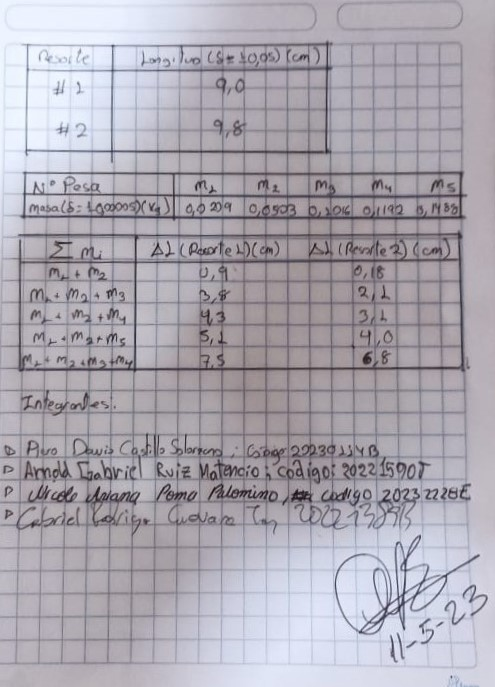
\includegraphics[width=0.6\linewidth]{images/anexo.jpg}
    \label{ref:anexo}
    \caption{Fotografía de la tabla de datos entregada al profesor.}
\end{figure}
\end{document}
